\chapter{Optimisation par les $\mathcal{H}$-matrices}
\label{hmatrixchapter}
Si on reconsidère l'algorithme~\ref{algo2} de la section~\ref{choleskySection1},
et que l'on pose $r = dm$, on rappelle la nécessité de connaître la factorisation de Cholesky $L$ de la
matrice de covariance $\Sigma~\in~M_{r}(\mathbb{R}) $ pour simuler $\mathcal{N}(0_{\mathbb{R}^{r}},\Sigma)$. Contrairement aux autres
opérations qui permettent la simulation, la méthode de Cholesky qui déduit
$L$ à partir de $\Sigma$ est très coûteuse: le nombre d'opérations est en
$\mathcal{O}(r^3)$. Ce temps nécessaire
pour déterminer $L$ sera appelé le coût de démarrage.\\
On devine clairement que pour un $r$ suffisament grand (de l'ordre de $10^3$), le coût
de démarrage devient non négligeable. Par conséquent, si on veut
simuler une gaussienne, il peut vite s'avérer judicieux de
réduire ce coût. De multiples façons existent pour le faire. On se propose ici
de présenter l'une d'elles qui consiste à considérer une structure de données
qui peut permettre dans certains cas la réduction du coût de démarrage. Il
s'agit de la structure des matrices hiérarchiques ou encore $\mathcal{H}$-matrices. Elles permettent des représentations compressées de matrices denses. Cette structure ne sera pas décrite dans les détails mais tout lecteur intéressé pourra se référer à la thèse de Benoît Lizé~\cite{LizéBenoît2014Rdrp}.

\section{Idée globale des $\mathcal{H}$-matrices}

L'idée de base de la structure des $\mathcal{H}$-matrices est de pouvoir
approcher certains blocs d'une matrice par 
des matrices de la forme $AB^{T}$. Une représentation de la forme $AB^{T}$ peut réduire
le coût mémoire de la matrice. En effet si on considère $A \in M_{m,k}(\mathbb{R})$ et $B \in M_{n,k}(\mathbb{R})$ où $k \leq  \min(m,n)$, alors stocker $AB^{T}$ coûte en mémoire
$mn$ cases-mémoire alors que stocker $A$ et $B$ coûte $k(m+n)$, ce qui peut être intéressant si $k \ll \min(m,n)$.

La représentation compressée d'une matrice dense $C$ en $\mathcal{H}$-matrice nécessite deux étapes: une subdivision en plusieurs blocs de la matrice $C$ (découpage hiérarchique) puis
on compresse au format $AB^{T}$ les blocs qui sont admissibles.

Une fois que l'on obtient la représentation compressée de la matrice, il sera possible de
faire diverses opérations élémentaires d'algèbre linéaire tout en préservant la
structure de $\mathcal{H}$-matrice. Dans le cas de la simulation d'un
champ gaussien, vu que l'algorithme de simulation est le même que l'algorithme~\ref{algo2} de la section~\ref{choleskySection1}, sauf que l'on utilise la structure des $\mathcal{H}$-matrices,
deux opérations seront différentes dans leur implémentation (qu'on n'évoquera pas): la factorisation de
Cholesky et le produit matrice-vecteur.

Pour la suite, pour $M \in M_{p,q}(\mathbb{R})$, $\sigma \subset \llbracket 1;p \rrbracket$,
$\tau \subset \llbracket 1;q \rrbracket$, on note $M_{|\sigma \times \tau}$ le
bloc $\sigma \times \tau$ de la matrice $M$, $(M_{i,j})_{(i,j) \in \sigma \times \tau}$. On dira aussi que $\sigma$ est un ensemble d'indices \og ligne\fg{} et que
$\tau$ est un ensemble d'indices \og colonne\fg{}.


\begin{figure}[h]
\begin{center}
\includegraphics[scale=0.6]{images/représentationCompressionHmatrice.jpg}
\caption{Compression au format $AB^{T}$}
\label{ideeCompressionHmatrice}  
\end{center}
\end{figure}

\section{Compression en $\mathcal{H}$-matrice}

\subsection{Découpage hiérarchique}

Dans cette sous-section, on emploiera du vocabulaire propre à la théorie
des graphes, notamment le concept d'arbre. \` A la page 66 de la thèse de Lizé,
il est possible de se familiariser avec ce vocabulaire.\\

Considérons $m,d$ et $N_{leaf}$ 3 entiers non nuls, $M \in M_{m}(\mathbb{R})$ une matrice carré. On suppose de plus qu'à chaque indice $j$ de l'ensemble
$\llbracket 1;m \rrbracket$, on associe un vecteur $x^j \in \mathbb{R}^d$ (dont on note sa $i$\up{ème} coordonnée $(x^j)_i$).  On peut voir les $x^j$ comme associés aux n\oe uds d'un maillage mais
on ne va pas jusqu'à supposer que les $x^i$ sont deux à deux distincts.
Notons par ailleurs $\mathcal{I}=\llbracket 1;m \rrbracket$.


\begin{remark}
\label{assignIndexLogic}
Si on réutilise les notations du chapitre~\ref{introProb} pour le temps de cette remarque et
que l'on reconsidère la matrice de covariance $\Sigma \in M_{dm}(\mathbb{R})$,
en raison de sa définition, pour chaque indice $i$ de l'ensemble
$\llbracket 1;dm \rrbracket$, on peut associer de façon logique un n\oe ud du maillage $M$.
En effet pour $i \in \llbracket 1; m \rrbracket, j \in \llbracket 1; d \rrbracket$,
on associe à l'indice $(i-1)m + j \in \llbracket 1;dm \rrbracket$, le n\oe ud $n_i$.
\end{remark}
\subsubsection{Découpage hiérarchique de l'espace}
\label{DecoupHieSpace}
\noindent Pour cette première étape, l'idée est de construire récursivement à partir de
la racine, un arbre $\mathcal{T}_{\mathcal{I}}$ dont les sommets sont des parties de $\llbracket 1;m \rrbracket$ (donc des ensembles d'indices).  L'arbre obtenu est un Cluster Tree (ou
arbre de groupes). La racine de l'arbre sera l'ensemble $\llbracket 1;m \rrbracket$. Afin de construire l'arbre, on a besoin d'une fonction
\og $\mathrm{Split}$ \fg{} qui à partir d'un ensemble d'indices $\sigma$, produit une partition de $\sigma$,
$\sigma_1, \cdots, \sigma_l$, où $l$ est en général fixé. Quand $l$ vaut $2$ on obtient un arbre binaire. Par ailleurs, on contraint à ce que toutes
les feuilles de $\mathcal{T}_{\mathcal{I}}$ soient des ensembles d'indices de cardinal
inférieur ou égal à $N_{leaf}$. \\ La construction du Cluster Tree est donnée par l'algorithme~\ref{algoClustTree} où pour
un sommet $\sigma$ de l'arbre, on notera $\mathrm{S}(\sigma)$ l'ensemble des fils
du sommet $\sigma$. Donc en particulier, si $\sigma$ est une feuille, $\mathrm{S}(\sigma)$ est l'ensemble vide.
\begin{remark}
Les feuilles de $\mathcal{T}_{\mathcal{I}}$ forment une partition de $\mathcal{I}$.   
\end{remark}


\begin{algorithm}
\caption{\textsc{Création du Cluster Tree}}
\label{algoClustTree}
\begin{algorithmic}
\STATE {\textbf{déf} createClusterTree($\sigma$) }
\STATE {\quad \textbf{si} $|\sigma| \leq N_{leaf}$ \textbf{alors} }
\STATE {\quad \quad $\mathrm{S}(\sigma) = \varnothing$ }
\STATE {\quad \textbf{sinon}}
\STATE {\quad \quad $\sigma_1, \cdots, \sigma_l = \mathrm{Split}(\sigma)$ }
\STATE {\quad \quad $\mathrm{S}(\sigma) = \{\sigma_1, \cdots, \sigma_l \}$}
\STATE {\quad \quad createClusterTree($\sigma_1$)}
\STATE {\quad \quad $\cdots$}
\STATE {\quad \quad createClusterTree($\sigma_l$)}
\END
\end{algorithmic}
\end{algorithm}

Pour la fonction \og $\mathrm{Split}$ \fg{} qui forme une partition, on évoquera deux choix possibles de fonction: le découpage
médian et le découpage géométrique. Si on considère $\sigma \subset \llbracket 1;m \rrbracket$, le début
des deux découpages est similaire: posons pour $i \in \llbracket 1;d \rrbracket$,
$x_{min,\sigma}^{i} = \min_{j \in \sigma} (x^j)_i $ et $x_{max,\sigma}^{i} = \max_{j \in \sigma} (x^j)_i $.
La première étape consiste à déterminer $i^{*} \in \llbracket 1;d \rrbracket$ tel que
$x_{max,\sigma}^{i^{*}} - x_{min,\sigma}^{i^{*}}$ soit de valeur maximale (on détermine donc l'axe où la boîte englobante
associée au $(x^j)_{j \in \sigma}$ est de largeur maximale).\\
La seconde étape produit la partition de
$\sigma$. Pour le découpage médian, on obtient la partition de $\sigma$, $\sigma_1$ et $\sigma_2$,
telle que si on note $x_{med,\sigma}^{i^{*}}$ la médiane de l'ensemble $\{(x^j)_{i^{*}}, j \in \sigma \}$, alors
pour $k \in \sigma$, $k$ est dans $\sigma_1$ si $(x^k)_{i^{*}} \leq x_{med,\sigma}^{i^{*}}$, sinon $k$ est dans $\sigma_2$.
Pour le découpage géométrique, on obtient la partition de $\sigma$, $\sigma_1$ et $\sigma_2$,
telle que si on note $x_{geo,\sigma}^{i^{*}} = (x_{min,\sigma}^{i^{*}} + x_{max,\sigma}^{i^{*}})/2$ alors
pour $k \in \sigma$, $k$ est dans $\sigma_1$ si $(x^k)_{i^{*}} \leq x_{geo,\sigma}^{i^{*}}$, sinon $k$ est dans $\sigma_2$.

\subsubsection{Découpage hiérarchique de la matrice}
\label{decoupHieMat}
Le découpage hiérarchique de la matrice consiste à construire à partir de $\mathcal{T}_{\mathcal{I}}$, un arbre
$\mathcal{T}_{\mathcal{I} \times \mathcal{I}}$ dont les sommets sont des parties de $\mathcal{I} \times \mathcal{I}$ de la forme $\sigma \times \tau$.
Ainsi, chaque sommet $\sigma \times \tau$ de l'arbre $\mathcal{T}_{\mathcal{I} \times \mathcal{I}}$ peut être associé au bloc $M_{|\sigma \times \tau}$
de la matrice $M$. Un tel arbre sera qualifié de Block Cluster Tree et la racine sera l'ensemble $\mathcal{I} \times \mathcal{I}$.
Pour décrire la construction de $\mathcal{T}_{\mathcal{I} \times \mathcal{I}}$,
il sera nécessaire d'introduire une fonction booléenne $f: \mathcal{P}(\mathcal{I}) \times \mathcal{P}(\mathcal{I}) \rightarrow \{0,1\}$
qui sera notre critère d'admissibilité. Plus exactement, on dira qu'un bloc $\sigma \times \tau$ est admissible si $f(\sigma,\tau) = 1$.
La construction de $\mathcal{T}_{\mathcal{I} \times \mathcal{I}}$ est décrite par l'algorithme~\ref{algoBlockClustTree} où la notation $\mathrm{S}(\sigma \times \tau)$
désignera les fils du sommet $\sigma \times \tau$ dans l'arbre $\mathcal{T}_{\mathcal{I} \times \mathcal{I}}$ tandis que la notation $\mathrm{S}(\sigma)$
désignera les fils du sommet $\sigma$ dans l'arbre $\mathcal{T}_{\mathcal{I}}$.

\begin{algorithm}
\caption{\textsc{Création du Block Cluster Tree}}
\label{algoBlockClustTree}
\begin{algorithmic}
\STATE {\textbf{déf} createClusterTree($\sigma \in \mathcal{T}_{\mathcal{I}}$, $\tau \in \mathcal{T}_{\mathcal{I}}$)}
\STATE {\quad \textbf{si} $f(\sigma,\tau) ==1$ ou $\mathrm{S}(\sigma) == \varnothing$ ou $\mathrm{S}(\tau) == \varnothing$  \textbf{alors} }
\STATE {\quad \quad $\mathrm{S}(\sigma \times \tau) = \varnothing$ }
\STATE {\quad \textbf{sinon}}
\STATE {\quad \quad $\mathrm{S}(\sigma \times \tau) = \{ \sigma^{\prime} \times \tau^{\prime},\; \sigma^{\prime} \in \mathrm{S}(\sigma) \text{ et } \tau^{\prime} \in \mathrm{S}(\tau) \}$ }
\STATE {\quad \quad \textbf{pour} $\sigma^{\prime} \times \tau^{\prime} \in \mathrm{S}(\sigma \times \tau)$ }
\STATE {\quad \quad \quad createClusterTree($\sigma^{\prime}$,$\tau^{\prime}$)}
\END
\end{algorithmic}
\end{algorithm}
  

Une fois que l'on obtient $\mathcal{T}_{\mathcal{I} \times \mathcal{I}}$, on remarque que si un sommet $\sigma \times \tau$ est admissible alors c'est une feuille.
On espère de façon générale que les feuilles admissibles soient des blocs de grande taille et que $N_{leaf}$ ait été choisi suffisamment petit
pour que les feuilles non admissibles soient de petites taille.
Finalement grâce à $\mathcal{T}_{\mathcal{I} \times \mathcal{I}}$, pour $\sigma \times \tau$ une feuille admissible, le bloc $M_{|\sigma \times \tau}$ de la matrice $M$
subira une compression pour être au format $AB^{T}$.\\

Pour la fonction booléenne $f$, son choix dépend du type de matrice que l'on considère et aussi du type de compression des blocs admissibles. On se contentera
donc d'exposer rapidement un critère d'admissibilité évoqué dans la thèse de Lizé. On définit pour $\sigma, \tau \subset \mathcal{I}$,
\begin{equation}
 \mathrm{diam}(\sigma)= \sqrt{\displaystyle\sum_{i=1}^{d} (x_{max,\sigma}^{i} - x_{min,\sigma}^{i})^2}
\end{equation}

\begin{equation}
 \mathrm{d}(\sigma,\tau) = \sqrt{\displaystyle\sum_{i=1}^{d} \max(0,x_{min,\tau}^{i} - x_{max,\sigma}^{i})^2 + \max(0,x_{min,\sigma}^{i} - x_{max,\tau}^{i})^2 } 
\end{equation}

\noindent $\mathrm{diam}(\sigma)$ désigne le diamètre de la boîte englobant les points $(x^j)_{j \in \sigma}$ et $\mathrm{d}(\sigma,\tau)$ désigne la
distance des faces les plus proches des deux boîtes englobantes associées à $\sigma$ et à $\tau$. Sous ces définitions,
il est maintenant possible de définir pour $\eta \in \mathbb{R}^{*}_{+}$ un critère d'admissibilité $f_{\eta}$: pour
$\sigma, \tau \subset \mathcal{I}$:
\begin{equation}
  \label{critAdmi}
  f_{\eta}(\sigma,\tau) =
  \begin{cases}
    1 & \quad \text{si } \min(\mathrm{diam}(\sigma),\mathrm{diam}(\tau)) < \eta \cdot \mathrm{d}(\sigma,\tau)\\
    0 & \quad \text{sinon}  \end{cases}
\end{equation}

\noindent $\eta$ est parfois appelé facteur d'admissibilité.\\


\begin{remark}
  Les feuilles de $\mathcal{T}_{\mathcal{I} \times \mathcal{I}}$ forment une partition de  $\mathcal{I} \times \mathcal{I}$. La représentation
  en $\mathcal{H}$-matrice consiste alors à stocker la matrice $M$ au niveau des feuilles de l'arbre $\mathcal{T}_{\mathcal{I} \times \mathcal{I}}$ où
  une feuille $\sigma \times \tau$ stockera aussi le sous-bloc $M_{|\sigma \times \tau}$ de la matrice $M$. Si de plus la feuille est admissible,
  alors on stockera $A$ et $B$ deux matrices issues de la compression et vérifiant $M_{|\sigma \times \tau} \approx AB^{T}$.
\end{remark}


\subsection{Compression des blocs admissibles}
\label{compBlocAdmi}
Si on considère $\sigma \times \tau$ un bloc admissible, alors on
espère que l'on dispose de $k \in \mathbb{N}^{*}$ vraiment plus petit que
$|\sigma|$ et $|\tau|$, de $A \in M_{|\sigma|,k}(\mathbb{R})$ et $B \in M_{|\tau|,k}(\mathbb{R})$ tels que $M_{|\sigma \times \tau} \approx AB^{T}$ au sens d'une norme
matricielle (on ne considérera que la norme spectrale $\|\cdot\|_2$ et la
norme de Frobenius $\|\cdot\|_F$). La représentation approchée de $M_{|\sigma \times \tau}$ par $AB^{T}$ est qualifiée de $\mathcal{R}k$-Matrice. Le théorème qui
suit présente la meilleure façon d'approcher une matrice par une
$\mathcal{R}k$-Matrice (SVD ou décomposition en valeurs singulières).

\begin{theorem}
  Soit $(p,q) \in (\mathbb{N}^{*})^2$, $A \in M_{p,q}(\mathbb{R})$. On
  note $A = U\Sigma V^{T}$ une décomposition en valeurs singulières de $A$ où
  $U \in M_{p,p}(\mathbb{R})$ et $V \in M_{q,q}(\mathbb{R})$ sont unitaires
  et $\Sigma \in M_{p,q}(\mathbb{R})$ est nulle sauf au niveau de sa diagonale
  et ses éléments diagonaux sont des réels positifs classés par ordre
  décroissant (ce sont les valeurs singulières).\\

  \noindent Soit $k \in \llbracket 1;\min(p,q) \rrbracket$. On note
  $\mathrm{diag}_{k}(\Sigma)$ la matrice $\Sigma$ où pour
  $i$ entier strictement plus grand que $k$,
  $\sigma_{i}=\Sigma_{i,i}$ a été remplacé par $0$.\\
  Alors si on note $\|\cdot\|$ la norme de Frobenius ou la norme spectrale,
  on a:
\begin{equation*}
\|A - U\mathrm{diag}_{k}(\Sigma)V^{T}\| = \min \{ \|A - R\|, \; R \in M_{p,q}(\mathbb{R}) \text{ tel que }\; \mathrm{rang}(R) \leq k \}
\end{equation*}
\noindent On a de plus:

\begin{equation}
  \label{approSpec}
\min \{ \|A - R\|_{2}, \; R \in M_{p,q}(\mathbb{R}) \text{ tel que }\; \mathrm{rang}(R) \leq k \} = \sigma_{k+1}^2
\end{equation}

\begin{equation}
  \label{approFrob}
\min \biggl \{ \|A - R\|_{F}^2, \; R \in M_{p,q}(\mathbb{R}) \text{ tel que }\; \mathrm{rang}(R) \leq k \biggr \} = \displaystyle\sum_{i=k+1}^{\min(p,q)} \sigma_{i}^2
\end{equation}
\end{theorem}


\begin{remark}
Les formules~(\ref{approSpec}) et~(\ref{approFrob}) montrent que
l'erreur d'approximation est complétement controlée par les valeurs singulières de $A$.
\end{remark}

\begin{remark}
On observe que $U\mathrm{diag}_{k}(\Sigma)V^{T}=PQ^{T}$ où $P=U\mathrm{diag}_{k}(\Sigma)$ et $Q=V$. D'où en plus d'être une $\mathcal{R}k$-Matrice,
$U\mathrm{diag}_{k}(\Sigma)V^{T}$ est une approximation optimale de $A$ par une matrice de rang au plus $k$.
Rajoutons que si on note $U_k \in M_{p,k}(\mathbb{R})$ (resp. $V_k \in M_{q,k}(\mathbb{R})$) la
matrice $U$ (resp. $V$) dont on ne retient que les $k$ premières colonnes. alors on a la représentation tronquée de rang $k$,
$U\mathrm{diag}_{k}(\Sigma)V^{T}= U_k\mathrm{diag}_{k}(\Sigma)V_{k}^{T} $, ce qui amène lorsque $k$ est connu à remplacer $U$ et $V$ par $U_k$ et $V_k$.\\
\end{remark}

En pratique, pour quantifier l'erreur, on utilise la norme de Frobenius et on a une quantité $\epsilon \in \mathbb{R}^{*}_{+}$ qui
est l'erreur absolue à ne pas dépasser. Ainsi si on reconsidère la matrice $A$ du théorème précédent, la méthode SVD conditionnée par $\epsilon$ consiste à déterminer
d'abord une décomposition en valeurs singulières (SVD)
de la matrice $A$ puis à choisir le rang $k$ comme étant le plus petit entier entre $1$ et $\min(p,q)$ tel que:
\begin{equation*} \|A - U\mathrm{diag}_{k}(\Sigma)V^{T}\|_{F} \quad = \quad \sqrt{\displaystyle\sum_{i=k+1}^{\min(p,q)} \sigma_{i}^2} \quad \leq \quad \epsilon \end{equation*}
Si les blocs admissibles sont compressés par la méthode SVD conditionnée par $\epsilon$, on appelle alors $\epsilon$ epsilon d'assemblage.\\
Cependant effectuer la SVD de la matrice $A$ admet une complexité en temps en $\mathcal{O}(pq^2 + p^2q)$. Donc compresser les blocs admissibles
par SVD pour obtenir pour chaque bloc une représentation tronquée conditionnée par l'erreur absolue $\epsilon$ peut s'avérer coûteux. C'est pourquoi il est préférable
d'opter pour un autre moyen de compression.\\

Les méthodes populaires de compression sont les méthodes ACA (Adaptive Cross Approximation). Ces méthodes
consistent à approcher une matrice $A \in M_{p,q}(\mathbb{R})$ par des approximations successives de rang $1$, $R_1 = C_1D_{1}^{T},  R_2 = C_2D_{2}^{T}, \cdots$
où les $C_i$ (resp. $D_i$) sont des vecteurs colonnes de taille $p$ (resp. de taille $q$)
et on cherche le plus petit entier $k$ vérifiant un certain critère d'arrêt pouvant être par exemple
\begin{equation} \|A - \displaystyle\sum_{i=1}^{k} R_i \|_{F} \leq \epsilon_1  \label{ACAcrit}\end{equation}
où $\epsilon_1 \in \mathbb{R}^{*}_{+}$ (appelé epsilon d'assemblage si on utilise ce critère pour compresser les blocs admissibles).
L'approximation de $A$, $\tilde{A}$, est définie ainsi \begin{equation*}\tilde{A} = \displaystyle\sum_{i=1}^{k} R_i \end{equation*}
$\tilde{A}$ est bien une $\mathcal{R}k$-Matrice car si on pose
\begin{equation*} C = \begin{pmatrix} C_1 & C_2 & \cdots & C_k \end{pmatrix} \text{ et } D = \begin{pmatrix}
    D_{1} & 0_{M_{q,1}(\mathbb{R})} & \cdots & 0_{M_{q,1}(\mathbb{R})} \\
    0_{M_{q,1}(\mathbb{R})} & D_{2} & \cdots & 0_{M_{q,1}(\mathbb{R})} \\
    \vdots & \vdots & \ddots & \vdots \\
    0_{M_{q,1}(\mathbb{R})} &  0_{M_{q,1}(\mathbb{R})} & \cdots & D_{k}
    \end{pmatrix}
   \end{equation*} alors \begin{equation*}\tilde{A} = CD^{T} \end{equation*}

Rajoutons qu'afin de réduire le rang de la matrice $\tilde{A}$ obtenue par une méthode ACA, il est possible d'appliquer une recompression de la matrice $\tilde{A}$
par une variante de la SVD (voir les pages de 58 à 60 de \cite{LizéBenoît2014Rdrp}). Dans cette variante, on applique un moment donné la méthode SVD conditionnée par un réel
strictement positif $\epsilon$ que l'on appelle epsilon de recompression.\\

Parmi les méthodes ACA, citons l'ACA pivotage total, l'ACA pivotage partiel, l'ACA+. Ces 3
méthodes sont évoquées dans la thèse de Lizé \cite{LizéBenoît2014Rdrp}.


\section{Complexité spatiale et temporelle}
L'algorithme~\ref{algo2} version $\mathcal{H}$-matrice pour une réalisation
nécessite plusieurs étapes: compresser en $\mathcal{H}$-matrice de la matrice de covariance $\Sigma \in M_{r}(\mathbb{R})$ où $r=dm$ (cette phase s'appelle aussi assemblage),
obtenir $L$, la factorisation de Cholesky version $\mathcal{H}$-matrice de $\Sigma$,
faire une réalisation $y$ du vecteur gaussien de loi $\mathcal{N}(0,I_{r})$,
et enfin faire le produit matrice-vecteur $Ly$.
~\\

La connaissance de la complexité en temps et en espace de ces étapes
permettrait d'obtenir celles de l'algorithme de simulation par
$\mathcal{H}$-matrice et on s'attend à ce qu'une forte compression de la matrice de
covariance réduise les coûts de temps et de mémoire. Cependant
cette compression dépend entre autres du type de matrices que l'on considère et
du découpage spatial. Par conséquent on ne peut donner de façon générale
la complexité en temps et en espace de l'algorithme~\ref{algo2} version $\mathcal{H}$-matrice pour une réalisation. Cependant en se référant à~\cite{LizéBenoît2014Rdrp},
on peut espérer pour certaines matrices une complexité spatiale de l'algorithme de simulation en $O(rlog(r))$ et une complexité temporelle en $O(r.log^2(r))$.

\begin{figure}[h]
\begin{center}
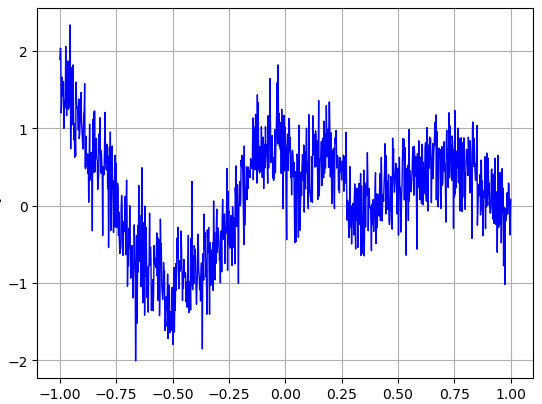
\includegraphics[scale=0.45]{images/hmatrixRea.jpg}
\caption{Réalisation sur $[-1,1]$ par méthode des $\mathcal{H}$-matrices}
\label{figHmatrixRea}  
\end{center}
\end{figure}

\newpage
\section{Erreur et convergence numérique}
\label{hmatrixerrconv}


\subsection{Paramétrage pour les tests}

Pour les tests numériques, la méthode des $\mathcal{H}$-matrices nécessite d'abord
l'information d'un maillage $M$ et d'une fonction de covariance $C$. Afin de comparer
cette méthode avec celle de Cholesky, on choisit que le choix des maillages pour
les dimensions 1, 2 et 3 et celui des fonctions de covariance seront les mêmes que ceux décrits
pour la méthode de Cholesky à la section~\ref{errConvCholesky} du chapitre~\ref{chapCholesky}. Cependant dans les sections précédentes on a vu que d'autres paramètres entraient en jeu,
en raison de la compression en $\mathcal{H}$-matrice de la
matrice de covariance $\Sigma \in M_{dm}(\mathbb{R})$. Pour que la compression soit possible, on
associe à chaque indice $i \in \llbracket 1;dm \rrbracket$ un n\oe ud du maillage $M$ en suivant la logique évoquée à la remarque~\ref{assignIndexLogic}. \\

Ces nouveaux paramètres ont été fixés de
façon identique pour tous les maillages et fonctions de covariance sélectionnés pour les tests: le paramètre $N_{leaf}$ (voir la sous-sous-section~\ref{DecoupHieSpace}) est fixé à $250$ et le type de découpage hiérarchique de l'espace sera le découpage médian. Pour le découpage
hiérarchique de la matrice (voir la sous-sous-section~\ref{decoupHieMat}), le critère
d'admissibilité (fonction booléenne) est la fonction définie par la formule~\eqref{critAdmi}
dont le facteur d'admissibilité $\eta$ est fixé à 100. Pour la compression des blocs
admissibles (voir la sous-section~\ref{compBlocAdmi}), on choisit la méthode ACA+
dont l'epsilon de recompression $\epsilon_1$ est fixé à $10^{-7}$ (voir formule~\eqref{ACAcrit}). Les blocs admissibles subiront après la méthode ACA+, une autre recompression par la
variante de la SVD où l'epsilon de recompression est fixé à $10^{-7}$.

\subsection{Benchmarks}

\begin{table}[htbp]
\centering
\begin{tabular}{|c |c |c |}
\hline
Dimension & Nb de n\oe uds & Temps moyen d'une réalisation (en seconde) \\
\hline
1 & 10 & 0.00014s    \\
\hline
1 & 100 & 0.00076s  \\
\hline
1 & 1000 & 0.07200s   \\
\hline
1 & 10000 & 0.55147s    \\
\hline
\hline
2 & 9 & 0.00024s    \\
\hline
2 & 100 & 0.00095s    \\
\hline
2 & 961 & 0.08200s  \\
\hline
2 & 10000 & 6.2282s   \\
\hline
\hline
3 & 8 & 0.00035s    \\
\hline
3 & 64 & 0.00063s    \\
\hline
3 & 729 & 0.07902s    \\
\hline
3 & 9261 & 60.024s  \\
\hline
\end{tabular}
\end{table}

\begin{table}[htbp]
\centering
\begin{tabular}{|c |c |c |c |c |}
\hline
Dimension & Nb de n\oe uds & Nb de réalisations  & erreur $L^2$ \\
\hline
1 & 10 & 250 & 0.16838   \\
\hline
1 & 10 & 500 &  0.11806   \\
\hline
1 & 10 & 750 &  0.10538   \\
\hline
1 & 10 & 1000 & 0.09248  \\
\hline
\hline
1 & 100 & 250 & 0.28641    \\
\hline
1 & 100 & 500 & 0.19507 \\
\hline
1 & 100 & 750 & 0.16492    \\
\hline
1 & 100 & 1000 & 0.13788    \\
\hline
\hline
1 & 1000 & 250 & 0.29194    \\
\hline
1 & 1000 & 500 & 0.22217    \\
\hline
1 & 1000 & 750 & 0.16064   \\
\hline
1 & 1000 & 1000 & 0.14545    \\
\hline
\hline
2 & 9 & 250 & 0.15007   \\
\hline
2 & 9 & 500 & 0.10969   \\
\hline
2 & 9 & 750 & 0.09103   \\
\hline
2 & 9 & 1000 & 0.07789  \\
\hline
\hline
2 & 100 & 250 & 0.44965   \\
\hline
2 & 100 & 500 & 0.31608   \\
\hline
2 & 100 & 750 & 0.25780    \\
\hline
2 & 100 & 1000 & 0.22462  \\
\hline
\hline
2 & 961 & 250 &  0.92465  \\
\hline
2 & 961 & 500 &  0.64501    \\
\hline
2 & 961 & 750 & 0.52958   \\
\hline
2 & 961 & 1000 & 0.45912    \\
\hline
\hline
3 & 8 & 250 & 0.15190  \\
\hline
3 & 8 & 500 & 0.09414   \\
\hline
3 & 8 & 750 & 0.08731    \\
\hline
3 & 8 & 1000 & 0.07096   \\
\hline
\hline
3 & 64 & 250 & 0.36302   \\
\hline
3 & 64 & 500 & 0.25823   \\
\hline
3 & 64 & 750 & 0.21156    \\
\hline
3 & 64 & 1000 & 0.18688    \\
\hline
\hline
3 & 729 & 250 & 1.1965   \\
\hline
3 & 729 & 500 & 0.84435   \\
\hline
3 & 729 & 750 & 0.69320   \\
\hline
3 & 729 & 1000 & 0.59755  \\
\hline
\end{tabular}
\end{table}

